\documentclass[onlytextwidth]{beamer}
\usepackage[utf8]{inputenc}
\usepackage{microtype}
\usepackage{amsmath}
\usepackage{amssymb}
\usepackage[nomessages]{fp} %\FPeval{\var-name}{2*sin(pi/6)}
\usepackage{siunitx} %units in math. eg 20\milli\meter
\usepackage{yhmath} % for arcs, overparenth command
\usepackage{tikz} %graphics
\usetikzlibrary{quotes, angles}
%\usepackage{graphicx} already loaded by beamer class
%consider setting \graphicspath{{images/}}
%\parskip ?? to avoid paragraph indent
\usepackage{multicol} %may not need this package, just columns environment
\usepackage{venndiagram}

\subtitle[BECA]{Bronx Early College Academy}
\author[Huson]{Christopher J. Huson PhD}

\setbeamertemplate{headline}{\vskip2mm 
  BECA / \insertshortauthor \, / \inserttitle
  \hfill 
  \insertsection
  }

\title{Geometry Unit 2: Angles}
\date{28 September - 7 October 2022}

\begin{document}
\frame{\titlepage}

\section[Outline]{}
\frame{\tableofcontents}

\section{2.1 Angle notation, measures \hfill 28 September}
\begin{frame}{Learning Target: I can measure angles}
  {CCSS: HSG.CO.A.1 Know precise geometric definitions \hfill \alert{2.1 Wednesday 28 Sept}}
  Do Now: Which takes longer, for a clock's hour hand to go from the 1 to the 4 or the 5 to the 9? \par \bigskip
    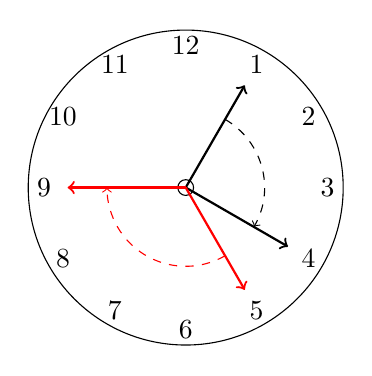
\begin{tikzpicture}
      \draw (0,0) circle [radius=2];
      \draw (0,0) circle [radius=0.1];
      \foreach \x in {1,...,12}
        \node at ({90+\x*-30}:1.8){\x};
      \draw[->, thick] (0,0)--(60:1.5);
      \onslide<2>
        \draw[->,thick] (0,0)--(-30:1.5);
        \draw[->,dashed] (60:1) arc (60:-30:1);
        \draw[->,thick,red] (0,0)--(-60:1.5);
        \draw[->,thick,red] (0,0)--(-180:1.5);
        \draw[->,dashed,red] (-60:1) arc (-60:-180:1);
    \end{tikzpicture} \par \bigskip
  Lesson: Angle measures, internal, external, acute, obtuse, right
\end{frame}

\begin{frame}{Two rays with a common endpoint make an \emph{angle}}
  Rays $\overrightarrow{BA}$ and $\overrightarrow{BC}$, \emph{vertex} $B$. \par \bigskip
    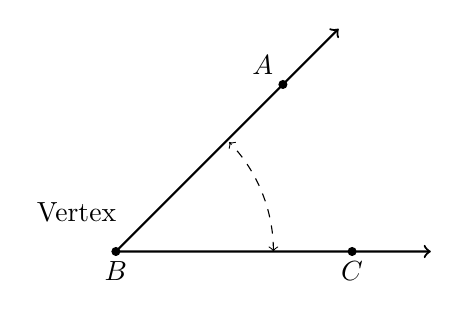
\begin{tikzpicture}
      \draw[<->, thick] (45:4)--(0,0)--(4,0);
      \draw[fill] (45:3) circle [radius=0.05] node[above left]{$A$};
      \draw[fill] (0,0) circle [radius=0.05] node[below]{$B$};
      \draw[fill] (3,0) circle [radius=0.05] node[below]{$C$};
      \node at (-0.5,0.5){Vertex};
      \onslide<2->{\draw[<->, dashed] (2,0) arc (0:44:2);}
    \end{tikzpicture}
    \begin{description}
      \item[Angle] Two rays with a common endpoint, $\angle ABC$ or $\angle B$
      \item[Vertex] The common end point of two rays making an angle
      \item[Interior] Inside, the area between the two rays
      \item[Exterior] Outside, the area in the angle interior 
      \onslide<2->{\item[m$\angle A$] The ``measure'' of angle $A$, how big it is}
    \end{description}
  \end{frame}

\begin{frame}{Babylonian measures: $360^\circ$ in a circle}
  \begin{center}
    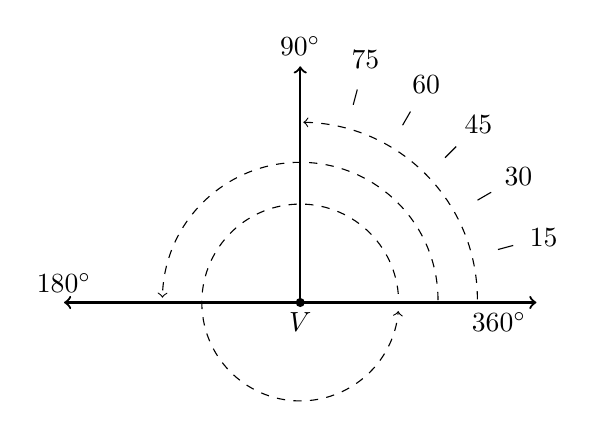
\begin{tikzpicture}
      \draw[<->, thick] (90:3)node[above]{$90^\circ$} --(0,0)--
        (3,0)node[below left]{$360^\circ$};
      \draw[->,thick] (0,0)--(-3,0)node[above]{$180^\circ$};
      \draw[fill] (0,0) circle [radius=0.05]node[below]{$V$};
      \draw[->,dashed] (1:2.25) arc (0:89:2.25);
      \draw[->,dashed] (1:1.75) arc (0:179:1.75);
      \draw[->,dashed] (5:1.25) arc (5:355:1.25);
      \onslide<2>
        {\foreach \x in {15,30,...,75}
          \node at (\x:3.2){\x};
        \foreach \x in {15,30,...,75}
          \draw (\x:2.6)--(\x:2.8);}
    \end{tikzpicture}
    \end{center}
  \begin{description}
    \item[Full turn] A complete rotation, $360^\circ$
    \item[Half turn] A straight line, $180^\circ$
    \item[Quarter turn] A \emph{right} angle, $90^\circ$
    \item[Protractor] A tool for measuring angles
  \end{description}
\end{frame}

\begin{frame}{Angle terminology and notation}
  {Write definitions in your notebook}
  \begin{columns}
    \column{0.4\textwidth}
    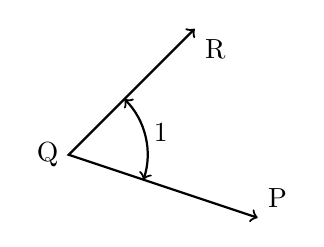
\begin{tikzpicture}[scale=0.8]
      \draw[<->, thick]
        (3,-1) coordinate (a) node[above right] {P}
        -- (0,0) coordinate (b) node[left] {Q}
        -- (2,2) coordinate (c) node[below right] {R}
        pic["1", <->, draw=black, angle eccentricity=1.2, angle radius=1cm]
        {angle=a--b--c};
    \end{tikzpicture}
    \column{0.6\textwidth}
    Angle $Q$, written $\angle Q$ (also $\angle PQR$, $\angle 1$) \par \medskip
    Point $Q$ is the \emph{vertex} \par \medskip
    The sides or \emph{legs} are $\overrightarrow{QR}$, $\overrightarrow{QP}$  \par \medskip
  \end{columns} \bigskip
  \begin{description}
    \item[Right angle] measuring $90^\circ$, mark as small square
    \tikz{\draw[<->] (0.5,0)--(0,0)--(0,0.5); \draw[thin] (0.3,0)--(0.3,0.3)--(0,0.3); }
    \item[Perpendicular] lines meet at right angles. $\overline{AB} \perp \overline{CD}$
    \item[Acute] angles measure $< 90^\circ$
    \item[Obtuse] angles are $90^\circ < \text{m}\angle < 180^\circ$
    \item[Straight angle] or a straight line  measures $180^\circ$
    \item[Reflex angles] measure $180^\circ < \text{m}\angle < 360^\circ$
  \end{description}
  \end{frame}

\section{2.2 Angle addition, angle pairs \hfill 29 September}
\begin{frame}{Learning Target: I can solve for angle measures}
  {CCSS: HSG.CO.A.1 Know precise geometric definitions \hfill \alert{2.2 Thursday 29 Sept}}
    Do Now: Given $\overline{LMN}$, $LM=2x-3$, $MN=x+7$, $LN=4x$. \par  
    Find $x$. \emph{Don't forget to check the solution.} \medskip 
      \begin{flushleft}
        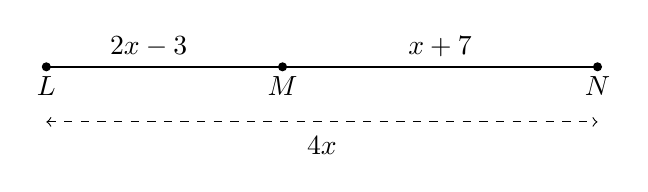
\begin{tikzpicture}
        \draw[thick] (0,0)--(7,0);
        \draw[fill] (0,0) circle [radius=0.05] node[below]{$L$};
        \draw[fill] (3,0) circle [radius=0.05] node[below]{$M$};
        \draw[fill] (7,0) circle [radius=0.05] node[below]{$N$};
        \node at (1.3,0) [above]{$2x-3$};
        \node at (5,0) [above]{$x+7$};
        \draw[<->, dashed] (0,-0.7)--(7,-0.7);
        \node at (3.5,-1){$4x$};
        \end{tikzpicture}
      \end{flushleft}
      \vspace{2cm}
    Name the geometry \emph{postulate} that is the basis for this problem. \par \medskip 
    Lesson: Angle addition postulate, complementary, supplementary angles, linear pairs
  \end{frame}

\begin{frame}{Angle addition postulate}
  $m\angle ABD=30^\circ$, $m\angle DBC=45^\circ$. Find $m\angle ABC$. \par \bigskip
    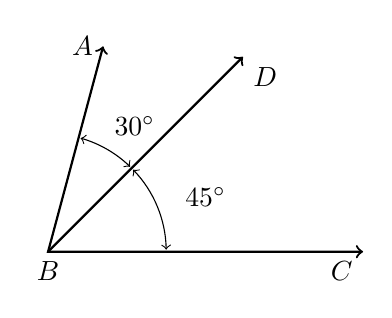
\begin{tikzpicture}
      \draw[<->, thick] (75:2.7) node[left]{$A$}--
        (0,0)node[below]{$B$}--
        (4,0) node[below left]{$C$};
      \draw[->, thick] (0,0)--(45:3.5)node[below right]{$D$};
      \draw[<->] (1:1.5) arc (1:44:1.5);
      \draw[<->] (46:1.5) arc (46:74:1.5);
      \node at (2,0.7){$45^\circ$};
      \node at (1.1,1.6){$30^\circ$};
    \end{tikzpicture} \vspace{1cm}
    \begin{description}
      \item[Angle addition] The sum of the measures of \emph{adjacent} angles is the measure of their combined angle. (postulate)
      \item[Adjacent] ``next to'' each other. Adjacent angles share a common ray and are external to each other.
    \end{description}
  \end{frame}

\begin{frame}{Special angle pairs}
  \begin{columns}
    \column{0.6\textwidth}
      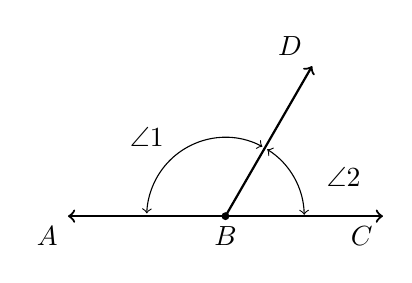
\begin{tikzpicture}
        \draw[<->, thick] (180:2) node[below left]{$A$}--
        (0,0)node[below]{$B$}--
        (2,0) node[below left]{$C$};
        \fill (0,0) circle [radius=0.05];
        \draw[->, thick] (0,0)--(60:2.2)node[above left]{$D$};
        \draw[<->] (1:1) arc (1:58:1);
        \draw[<->] (62:1) arc (62:178:1);
        \node at (-1,1){$\angle 1$};
        \node at (1.5,0.5){$\angle 2$};
        \end{tikzpicture} \par 
      Linear pair, supplementary $\angle$s
    \column{0.4\textwidth}
      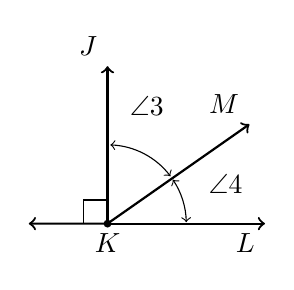
\begin{tikzpicture}
        \draw[<->, thick] (90:2) node[above left]{$J$}--
        (0,0)node[below]{$K$}--
        (2,0) node[below left]{$L$};
        \fill (0,0) circle [radius=0.05];
        \draw[<->, thick] (-1,0)--(0,0)--(35:2.2)node[above left]{$M$};
        \draw (0,0)++(-0.3,0)--++(0,0.3)--++(0.3,0);
        \draw[<->] (1:1) arc (1:34:1);
        \draw[<->] (37:1) arc (37:88:1);
        \node at (0.5,1.5){$\angle 3$};
        \node at (1.5,0.5){$\angle 4$};
      \end{tikzpicture} \par 
      Complementary angles
  \end{columns} \vspace{0.7cm}
    \begin{description}
      \item[Linear pair] Two adjacent angles that make a straight line
      \item[Opposite rays] collinear with a common endpoint. $\overrightarrow{BA}$, $\overrightarrow{BC}$
      \item[Supplementary] Angles whose measures sum to $180^\circ$
      \item[Complementary] Angles whose measures sum to $90^\circ$
      \item[Adjacent] ``next to'' each other. Adjacent angles share a common ray and are external to each other.
    \end{description}
\end{frame}

\begin{frame}{Given two supplementary angles, a linear pair.}
  m$\angle ABD = 4x+16$, m$\angle CBD = 100$. Find $x$. \vspace{1cm}
  \begin{columns}
    \column{0.5\textwidth}
      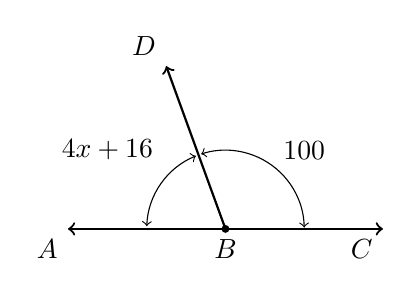
\begin{tikzpicture}
        \draw[<->, thick] (180:2) node[below left]{$A$}--
        (0,0)node[below]{$B$}--
        (2,0) node[below left]{$C$};
        \fill (0,0) circle [radius=0.05];
        \draw[->, thick] (0,0)--(110:2.2)node[above left]{$D$};
        \draw[<->] (1:1) arc (1:108:1);
        \draw[<->] (112:1) arc (112:178:1);
        \node at (-1.5,1){$4x+16$};
        \node at (1,1){$100$};
        \end{tikzpicture} \par 
    \column{0.5\textwidth} 
      \onslide<2->{
        Solution: 
        $$\text{m}\angle ABD + \text{m}\angle CBD = 180$$ }
        \onslide<3>{
        $$(4x+16) + 100 = 180$$
        $$\dots$$
        $$x=16$$
        Check: \par
        $[4(16)+16] + 100 = 180$ \checkmark
        }
    \end{columns} \vspace{1cm}
  \end{frame}

\begin{frame}{Extension (optional problems)}
  At midnight both the clock's minute hand and hour hand point at the same direction. When is the next time the clock hands coincide? \par \bigskip
    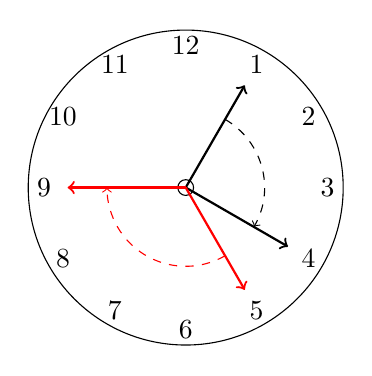
\begin{tikzpicture}
      \draw (0,0) circle [radius=2];
      \draw (0,0) circle [radius=0.1];
      \foreach \x in {1,...,12}
        \node at ({90+\x*-30}:1.8){\x};
      \draw[->, thick] (0,0)--(60:1.5);
      \onslide<2>
        \draw[->,thick] (0,0)--(-30:1.5);
        \draw[->,dashed] (60:1) arc (60:-30:1);
        \draw[->,thick,red] (0,0)--(-60:1.5);
        \draw[->,thick,red] (0,0)--(-180:1.5);
        \draw[->,dashed,red] (-60:1) arc (-60:-180:1);
    \end{tikzpicture}
  \end{frame}

\section{2.3 Vertical angles \hfill 30 September}
\begin{frame}{Learning Target: I can identify vertical angles}
  {CCSS: HSG.CO.A.1 Know precise geometric definitions  \hfill \alert{2.3 Friday 30 September}}
  
    Definition: \emph{Vertical angles} are angles opposite each other when two lines intersect. $\angle 1$ and $\angle 3$ are vertical angles, as are $\angle 2$ and $\angle 4$.
  \begin{center}
  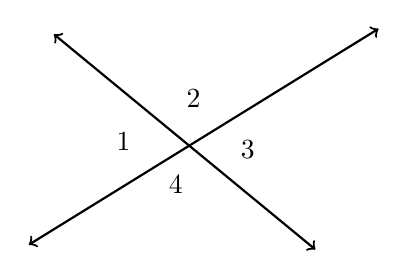
\begin{tikzpicture}[scale=0.5, rotate=15]
    \draw[<->, thick] (0,-1.5)--(10,1.5);
    \draw[<->, thick] (2,3.5)--(7,-3.5);
    \node at (3,.4){1};
    \node at (6,-.6){3};
    \node at (5,1){2};
    \node at (4,-1){4};
    %\draw[fill] (0,0) circle [radius=0.05] node[below]{$P$};
    %\draw[fill] (6,0) circle [radius=0.05] node[below]{$R$};
    %\draw[fill] (3,0) circle [radius=0.05] node[below]{$Q$};
  \end{tikzpicture}
  \end{center}
    Lesson: Vertical angles
  \end{frame}
  
\begin{frame}{Write down definitions in your notebook}
  \begin{block}{Angle pairs}
  \begin{enumerate}
      \item \emph{Adjacent} angles share a leg (``next to each other'')
      \item \emph{Complementary} angles measures sum to $90^\circ$
      \item \emph{Supplementary} angles sum to $180^\circ$
      \item \emph{Vertical} or opposite angles made by intersecting lines (1, 2)
      \item \emph{Linear pairs}, adjacent angles making a straight line (3, 4)
  \end{enumerate}
  \end{block}
  \begin{multicols}{2}
  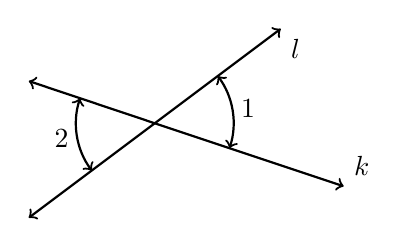
\begin{tikzpicture}[scale=0.8]
    \draw[<->, thick]
      (3,-1) coordinate (a) node[above right] {$k$}
      -- (0,0) coordinate (b) %node[left] {Q}
      -- (2,1.5) coordinate (c) node[below right] {$l$}
      pic["1", <->, draw=black, angle eccentricity=1.2, angle radius=1cm]
      {angle=a--b--c};
      \draw[<->, thick]
      (-2,0.67) coordinate (d) %node[right] {P}
      -- (0,0) coordinate (e) %node[left] {Q}
      -- (-2,-1.5) coordinate (f) %node[above right] {R}
      pic["2", <->, draw=black, angle eccentricity=1.2, angle radius=1cm]
      {angle=d--e--f};
  \end{tikzpicture}
  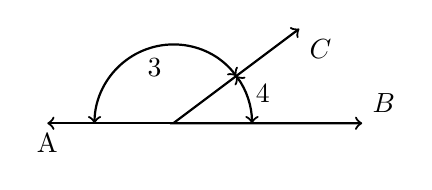
\begin{tikzpicture}[scale=0.8]
    \draw[<->, thick]
      (3,0) coordinate (a) node[above right] {$B$}
      -- (0,0) coordinate (b) %node[left] {Q}
      -- (2,1.5) coordinate (c) node[below right] {$C$}
      pic["4", <->, draw=black, angle eccentricity=1.2, angle radius=1cm]
      {angle=a--b--c};
      \draw[<-, thick]
      (-2,0) coordinate (d) node[below] {A}
      -- (0,0) coordinate (e)
      pic["3", <->, draw=black, angle eccentricity=0.75, angle radius=1cm]
      {angle=c--e--d};
  \end{tikzpicture}
  \end{multicols}
  \end{frame}
  
\begin{frame}{Angle pairs: check your knowledge}
  \begin{enumerate}
    \item \emph{Complementary} angles sum to how many degrees?
    \item \emph{Supplementary} angles sum to how many degrees?
    \item Given complementary angles $\angle A$ and $\angle B$ with $m\angle A = 30^\circ$. Find $m\angle B$. \vspace{0.25cm}
    \item Given $m\angle A = 100^\circ$ and $m\angle B = 2x$. Find $x$ such that angles $\angle A$ and $\angle B$ are supplementary.  \vspace{0.75cm}
    \begin{multicols}{2}
      \item Given vertical angles as shown. Find $x$. \\
      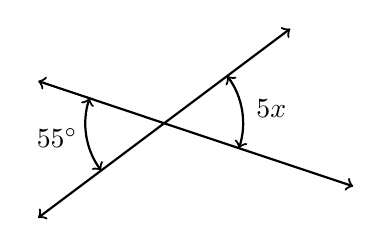
\begin{tikzpicture}[scale=0.8]
        \draw[<->, thick]
          (3,-1) coordinate (a) %node[above right] {$k$}
          -- (0,0) coordinate (b) %node[left] {Q}
          -- (2,1.5) coordinate (c) %node[below right] {$l$}
          pic["$\quad 5x$", <->, draw=black, angle eccentricity=1.2, angle radius=1cm]
          {angle=a--b--c};
          \draw[<->, thick]
          (-2,0.67) coordinate (d) %node[right] {P}
          -- (0,0) coordinate (e) %node[left] {Q}
          -- (-2,-1.5) coordinate (f) %node[above right] {R}
          pic["$55^\circ \quad$", <->, draw=black, angle eccentricity=1.2, angle radius=1cm]
          {angle=d--e--f};
      \end{tikzpicture}
    \end{multicols}
    \end{enumerate} \vspace{1cm}
  \end{frame}

\begin{frame}{Angle pairs: apply your knowledge}
  \begin{block}{Triangle external angle situation}
    \begin{center}
    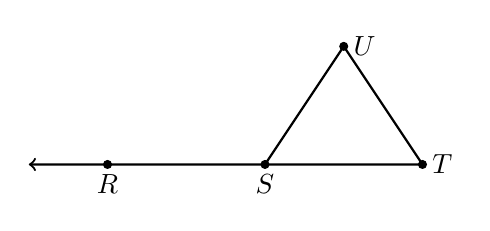
\begin{tikzpicture}
      %\draw[->, thick] (0,0)--(5,5);
      \draw[<-, thick] (-2,0)--(3,0)--(2,1.5)--(1,0);
      \draw[fill] (-1,0) circle [radius=0.05] node[below]{$R$};
      \draw[fill] (1,0) circle [radius=0.05] node[below]{$S$};
      \draw[fill] (2,1.5) circle [radius=0.05] node[right]{$U$};
      \draw[fill] (3,0) circle [radius=0.05] node[right]{$T$};
    \end{tikzpicture}
    \end{center}
    \begin{enumerate}
      \item Given $m\angle RSU = 115^\circ$. Find $m\angle TSU$
      \item Given $S$ bisects $\overline{RT}$, $RS=\frac{1}{5} (x+8)$ and $ST = x$. Find $RT$.
  \end{enumerate}
  \end{block}
  \end{frame}
  
\begin{frame}{Write down definitions in your notebook}
  \begin{block}{A postulate is a fundamental statement we agree is true}
  \begin{enumerate}
      \item \emph{Scalene} triangles have three unequal sides
      \item \emph{Horizontal}, sideways or level
      \item \emph{Vertical}, straight up and down
      \item An angle's \emph{measure}, it's size, is written $m \angle$
      \begin{multicols}{2}
        \item \emph{Angle Addition Postulate}\\ Measures of adjacent angles sum to the resulting angle \\[0.25cm]
        $m\angle 1 + m\angle 2 = m \angle ABC$ \\
        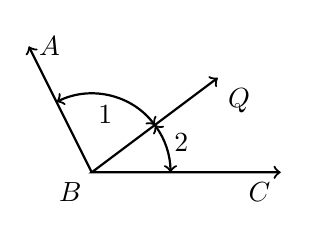
\begin{tikzpicture}[scale=0.8]
          \draw[<->, thick]
            (3,0) coordinate (a) node[below left] {$C$}
            -- (0,0) coordinate (b) node[below left] {$B$}
            -- (2,1.5) coordinate (c) node[below right] {$Q$}
            pic["2", <->, draw=black, angle eccentricity=1.2, angle radius=1cm]
            {angle=a--b--c};
            \draw[<-, thick]
            (-1,2) coordinate (d) node[right] {$A$}
            -- (0,0) coordinate (e)
            pic["1", <->, draw=black, angle eccentricity=0.75, angle radius=1cm]
            {angle=c--e--d};
        \end{tikzpicture}
      \end{multicols}
        \end{enumerate}
  \end{block} \vspace{1cm}
\end{frame}


\section{2.4 Angle bisectors \hfill 3 October}
\begin{frame}{Learning Target: I can bisect angles}
  {CCSS: HSG.CO.A.1 Know precise geometric definitions  \hfill \alert{2.4 Monday 3 October}}
  Do Now: Given vertical angles measuring $4x+4$ and $52^\circ$. Find $x$. \par \bigskip
  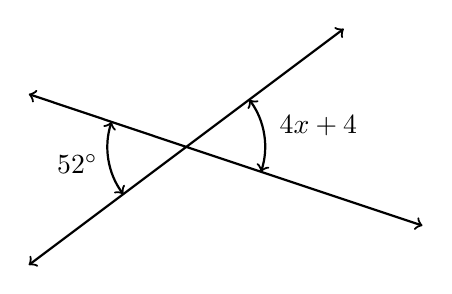
\begin{tikzpicture}[scale=1]
    \draw[<->, thick]
      (3,-1) coordinate (a) %node[above right] {$k$}
      -- (0,0) coordinate (b) %node[left] {Q}
      -- (2,1.5) coordinate (c) %node[below right] {$l$}
      pic["$4x+4$", <->, draw=black, angle eccentricity=1.7, angle radius=1cm]
      {angle=a--b--c};
      \draw[<->, thick]
      (-2,0.67) coordinate (d) %node[right] {P}
      -- (0,0) coordinate (e) %node[left] {Q}
      -- (-2,-1.5) coordinate (f) %node[above right] {R}
      pic["$52^\circ$", <->, draw=black, angle eccentricity=1.4, angle radius=1cm]
      {angle=d--e--f};
  \end{tikzpicture} \par \bigskip
  Lesson: Angle bisector situations
  \end{frame}

\begin{frame}{Bisect an angle by dividing it exactly in half}
    $\overrightarrow{BD}$ bisects $\angle ABC$ if and only if $\angle ABD \cong \angle CBD$. \par \bigskip
    \begin{center}
      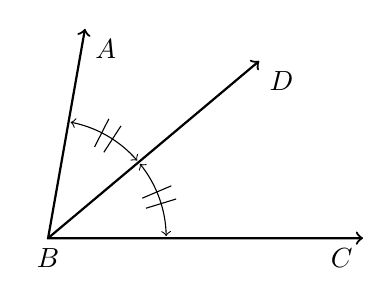
\begin{tikzpicture}
        \draw[<->, thick] (80:2.7) node[below right]{$A$}--
          (0,0)node[below]{$B$}--
          (4,0) node[below left]{$C$};
        \draw[->, thick] (0,0)--(40:3.5)node[below right]{$D$};
        \draw[<->] (1:1.5) arc (1:39:1.5);
        \draw (17:1.3)--(17:1.7);
        \draw (23:1.3)--(23:1.7);
        \draw[<->] (41:1.5) arc (41:79:1.5);
        \draw (57:1.3)--(57:1.7);
        \draw (63:1.3)--(63:1.7);
      \end{tikzpicture} 
      \end{center}
      \begin{description}
        \item[Angle bisector] ray dividing an angle into two congruent angles
        \item[Hash marks] mark congruent angles
      \end{description}
    \end{frame}

\begin{frame}{Model angle situations with algebra, then solve}
  Given angle bisector $\overrightarrow{BD}$ with m$\angle ABD =60^\circ$ and m$\angle CBD=2x+10$. Find $x$.
  \begin{columns}
    \column{0.6\textwidth}
    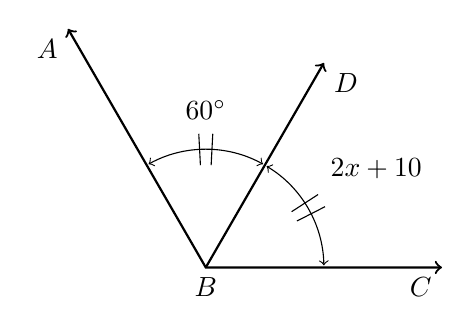
\begin{tikzpicture}
      \draw[<->, thick] (120:3.5) node[below left]{$A$}--
        (0,0)node[below]{$B$}--
        (3,0) node[below left]{$C$};
      \draw[->, thick] (0,0)--(60:3)node[below right]{$D$};
      \draw[<->] (1:1.5) arc (1:59:1.5);
      \draw (27:1.3)--(27:1.7);
      \draw (33:1.3)--(33:1.7);
      \draw[<->] (61:1.5) arc (61:119:1.5);
      \draw (87:1.3)--(87:1.7);
      \draw (93:1.3)--(93:1.7);
      \node at (30:2.5){$2x+10$};
      \node at (90:2){$60^\circ$};
    \end{tikzpicture} 
    \column{0.4\textwidth}
    \onslide<2>
    Solution:
    $$\angle ABD \cong \angle CBD$$
    $$2x+10=60$$
    $$2x=50$$
    $$x=25$$
    Check: \par
    $2(25)+10=60$? \checkmark
  \end{columns}
  \end{frame}  

\begin{frame}{Extension: Use angles for compass directions}
  {North South East West, \href{https://en.wikipedia.org/wiki/Points_of_the_compass}{points of the compass}}
  Directions are measured relative to North \bigskip
  \begin{columns}
    \column{0.5\textwidth}
    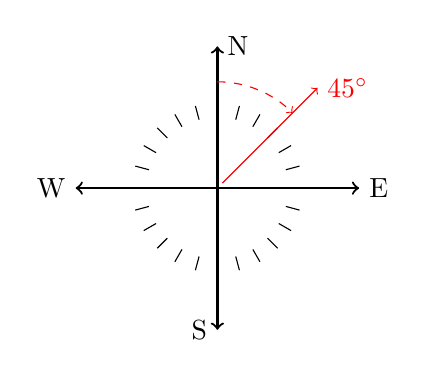
\begin{tikzpicture}[scale=0.9]
      \draw[<->,thick] (-2,0)node[left]{W}--(2,0)node[right]{E};
      \draw[<->,thick] (0,-2)node[left]{S}--(0,2)node[right]{N};
      \foreach \x in {1,...,24}
        \draw ({\x*15}:1)--({\x*15}:1.2);
    \onslide<2->
      \draw[->,dashed,red] (90:1.5) arc (90:45:1.5);
      \draw[->,red] (45:0.1)--(45:2)node[right]{$45^\circ$};
    \end{tikzpicture} 
    \column{0.5\textwidth}
    \onslide<2->{
    ``Northeast,'' half way between north and east, i.e. bearing $45^\circ$ \par \bigskip
    north is $0^\circ$ \par 
    east is $90^\circ$ \par 
    south is $180^\circ$ \par 
    west is $270^\circ$ \par }
  \end{columns} \bigskip
  \begin{description}
    \item[Bearing] The direction as an angle \emph{clockwise} from north
    \item[Clockwise] The direction the clocks turn, ``to the right'' (tighten)
    \item[Counterclockwise] Opposite of clocks, ``to the left'' (loosen)
  \end{description}
  \end{frame}  

\section{2.5 Triangle sum; equilateral, isosceles $\triangle$ angles \hfill 4 October}
\begin{frame}{LT: I can work with equilateral and isosceles-right $\triangle$s}
  {CCSS: HSG.CO.A.1 Know precise geometric definitions  \hfill \alert{2.5 Tuesday 4 October}}
  Do Now: Given perpendiculars $\overrightarrow{AB} \perp \overleftrightarrow{BC}$, and that the ray $\overrightarrow{BD}$ bisects $\angle ABC$, making two angles, $\angle 1$ and $\angle 2$. \par \medskip
  Find the measures of $\angle 1$, $\angle 2$.
  \begin{flushleft}
    \begin{tikzpicture}
      \draw[<->, thick] (-2,0)--(0,0)--(4,0);
      \draw[->, thick] (0,0)--(90:3);
      \draw[->, dashed] (0,0)--(45:4);
      \draw (0,0)++(-0.3,0)--++(0,0.3)--++(0.3,0);
      \node at (1.2,0.5){$1$};
      \node at (0.4,1.2){$2$};
      \draw[fill] (45:3) circle [radius=0.05] node[below right]{$D$};
      \draw[fill] (90:2.5) circle [radius=0.05] node[left]{$A$};
      \draw[fill] (0,0) circle [radius=0.05] node[below]{$B$};
      \draw[fill] (3,0) circle [radius=0.05] node[below]{$C$};
    \end{tikzpicture}
    \end{flushleft}
    Lesson: Isosceles base theorem, special triangles \par $60^\circ$ - $60^\circ$ - $60^\circ$, $30^\circ$ - $60^\circ$ - $90^\circ$, $45^\circ$ - $45^\circ$ - $90^\circ$
  \end{frame}

\begin{frame}{Equilateral $\triangle$, special relationships and measures}
  \begin{columns}
  \column{0.5\textwidth}
    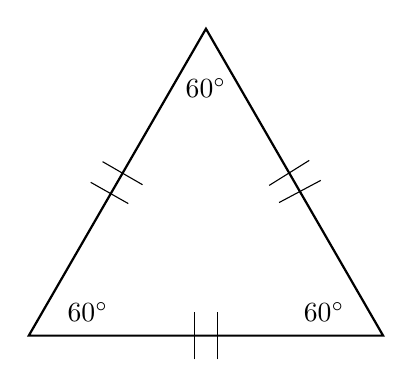
\begin{tikzpicture}[scale=1.5]
      \draw[thick] (0,0)--(3,0)--(60:3)--cycle;
      \draw (1.4,-0.2)--(1.4,0.2);
      \draw (1.6,-0.2)--(1.6,0.2);
      \draw (53:1.4)--(68:1.4);
      \draw (53:1.6)--(67:1.6);
      \draw (28:2.4)--(28:2.8);
      \draw (32:2.4)--(32:2.8);
      \node at (0.5,0.2){$60^\circ$};
      \node at (1.5,2.1){$60^\circ$};
      \node at (2.5,0.2){$60^\circ$};
    \end{tikzpicture}
    \center{$60^\circ$ - $60^\circ$ - $60^\circ$}
  \column{0.5\textwidth}
  \onslide<2->
    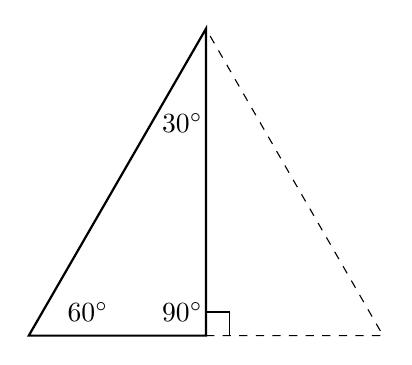
\begin{tikzpicture}[scale=1.5]
      \draw[thick] (0,0)--(1.5,0)--(60:3)--cycle;
      \draw[dashed] (1.5,0)--(3,0)--(60:3);
      \node at (0.5,0.2){$60^\circ$};
      \node at (1.3,1.8){$30^\circ$};
      \node at (1.3,0.2){$90^\circ$};
      \draw (1.5,0)++(0.2,0)--++(0,0.2)--++(-0.2,0);
    \end{tikzpicture} \par
    \center{$30^\circ$ - $60^\circ$ - $90^\circ$}
  \end{columns} \vspace{1cm}
  \begin{description}
    \item[Equiangular] means having equal angles
    \item[Equilateral] having equal sides 
  \end{description}
  \end{frame}

\begin{frame}{Isosceles-right triangles' angles measure $45^\circ$ - $45^\circ$ - $90^\circ$}
  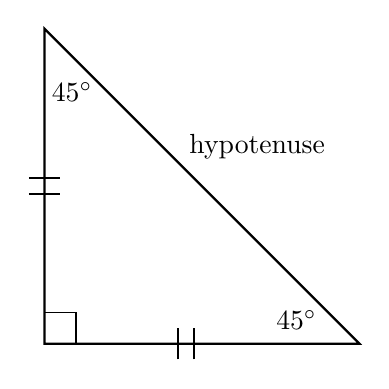
\begin{tikzpicture}[scale=1]
    \draw[thick](0,0)--(4,0)--(0,4)--cycle;
    \draw (0,0)++(0.4,0)--++(0,0.4)--++(-0.4,0);
    \node at (3.2,0.3){$45^\circ$};
    \node at (0.35,3.2){$45^\circ$};
    \node at (2.7,2.5){hypotenuse};
    \draw[thick] (1.7,-0.2)--(1.7,0.2);
    \draw[thick] (1.9,-0.2)--(1.9,0.2);
    \draw[thick] (-0.2,1.9)--(0.2,1.9);
    \draw[thick] (-0.2,2.1)--(0.2,2.1);
  \end{tikzpicture} \vspace{1cm}
  \begin{description}
    \item[Hypotenuse] the longest side of a right triangle, opposite the $90^\circ$ angle 
  \end{description}
  \end{frame}

\section{2.6 Review \hfill 6 October}
\begin{frame}{Angle relationships}
  Review: Angle postulates and theorems you have learned. 
  \begin{enumerate}
    \item $\perp$ lines and complementary $\angle$s make $90^\circ$
    \item linear pairs add to $180^\circ$
    \item vertical $\angle$s are $\cong$
    \item definition of an angle bisector
    %\item isosceles base angle theorem
  \end{enumerate}
\end{frame}

\section{2.7 Test: Angle measures \hfill 7 October}

\section{Open Middle: complementary and supplementary puzzle}
\begin{frame}{Open Middle problem (fun)}
  {Use digits from 0 to 9. Using a digit no more than once.}
    \begin{block}{The first two angle measures are complementary. The second two angles supplementary. (degrees)}
      \begin{center}
        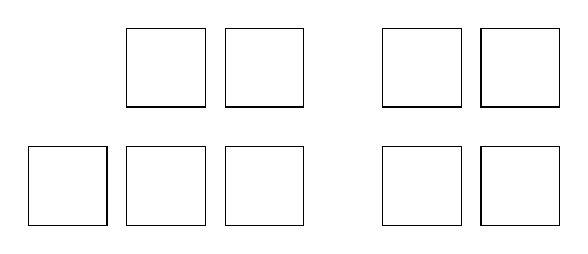
\begin{tikzpicture}
        \draw (0,0) rectangle (1,1);
        \draw (1.25,0) rectangle (2.25,1);
        \draw (3.25,0) rectangle (4.25,1);
        \draw (4.5,0) rectangle (5.5,1);

        \draw (-1.25,-1.5) rectangle (-0.25,-0.5);
        \draw (0,-1.5) rectangle (1,-0.5);
        \draw (1.25,-1.5) rectangle (2.25,-0.5);
        \draw (3.25,-1.5) rectangle (4.25,-0.5);
        \draw (4.5,-1.5) rectangle (5.5,-0.5);
     \end{tikzpicture}
    \end{center}
    \end{block} \vspace{1cm} 
\end{frame}


\end{document}